\subsection{Особенности детектора RICH эксперимента CBM}\label{sec:secCBMrich}

% \textbf{Эта секция пока что выглядит сыровато. Надо смержить с наиболее объёмным вариантом статьи. Надо написать, среди прочего, мотивировку к обеим темам диссера --- ДАК и Билдер! Ещё в секции флес-дак первой части первой главы надо упомянуть, что бестриггерная схема --- это новшество, которое требует испытаний прототипов.}

% Из диссера Копфера

% For SIS100 the background is already dominated by physical sources like $\gamma$-conversion in the target or $\pi^{0}$-Dalitz decays at a pion suppression factor of $10^3$ (see section 2.6). The electron identification covers the full angular acceptance of the CBM detector, i.e. from \SI{2.5}{\degree} to \SI{25}{\degree} in polar angle and full azimuthal coverage. In order to accommodate the bending of tracks in the dipole magnet, all detectors behind the magnetic field will be wider by a factor 1.5 compared to the height.

Конструкция и компоновка детектора черенковских колец эксперимента CBM подвергается постоянной оптимизации. Ниже рассмотрена версия, актуальная на момент написания данной диссертации. Значительная часть выполненных к настоящему времени работ по оптимизации описана в главе 3. Разработке и исследованиям прототипа системы считывания CBM RICH в составе полнофункционального прототипа детектора RICH посвящены главы~4~и~5. % \todo проверить номера

Аксептанс детектора, с учётом расширения по горизонтали из-за наличия магнитного поля, разводящего частицы, представляет собой конус \SI{0}{\degree}--\SI{25}{\degree} с вершиной в точке первичного взаимодействия, растянутый по горизонтали в 1.5 раза. Таким образом в плоскости ZX угол составляет \SI{0}{\degree}--\SI{37.5}{\degree}.
% Аксептанс детектора составляет $\SI{25}{\degree}$ по вертикали и $\SI{37.5}{\degree}$ по горизонтали.

Продольный размер RICH-детектора определяется доступным пространством между кремниевой трековой системой STS, расположенной внутри магнита, и детектором переходного излучения TRD. С одной стороны, высокая длина радиатора предпочтительна, т.к. она определяет высокий выход черенковских фотонов. С другой стороны, чем меньше расстояние между последней станцией STS и первой станцией TRD, тем выше эффективность трекинга. Не последнее значение имеют финансовые аргументы. Уменьшение длины детектора означает уменьшение размеров фоточувствительной камеры, следовательно уменьшение количества фотодетекторов и уменьшение площади зеркал, то есть снижение стоимости прибора.
Из этих соображений для RICH отведено пространство от 1800~мм до 3700~мм по оси пучка, не ограниченное по другим осям ничем, кроме пола. Длина этого пространства вдоль оси пучка составляет 1900~мм. Перед RICH и за ним отведено ещё по 100~мм общего пространства для стыковки магнита, STS, RICH и пучковой трубы. Зеркало расположено на расстоянии 3500~мм от точки взаимодействия, таким образом, рабочая длина радиатора составляет 1700~мм. Исходя из того факта, что зеркала должны полностью покрывать геометрический аксептанс, ширина детектора выбрана 5268~мм, а высота 4420~мм.

CBM RICH будет иметь корпус из алюминия толщиной 5~мм. Передняя и задняя стенки, находящиеся в аксептансе, будут выполнены из каптона толщиной 250~мкм для снижения толщины материала~\cite{TDR_RICH}.

% Нужна ли такая ссылка?

% Original English text
% The radiator length is 1.7~m and the volume $\approx 35 m^{3}$. Since the RICH detector will be placed between the STS in the dipole magnet and the TRD detector, its overall length is constrained by the distance between the magnet and its shielding yokes at about 1.6~m from target and the first TRD station. On the one hand, a long radiator is favourable due to the proportionality between photon yield and radiator length according to equation (2.8). On the other hand, a short gap between the tracking detectors STS and TRD is advantageous for tracking which requires a short RICH detector in between. In consequence, the overall length of the RICH detector including radiator, mirror, and support structure is foreseen to be $\approx 2$~m.

\textbf{ТУТ РАНО ИЛИ ПОЗДНО БУДЕТ КРАСИВАЯ КАРТИНКА}
%\begin{figure}[H]
%\centering
%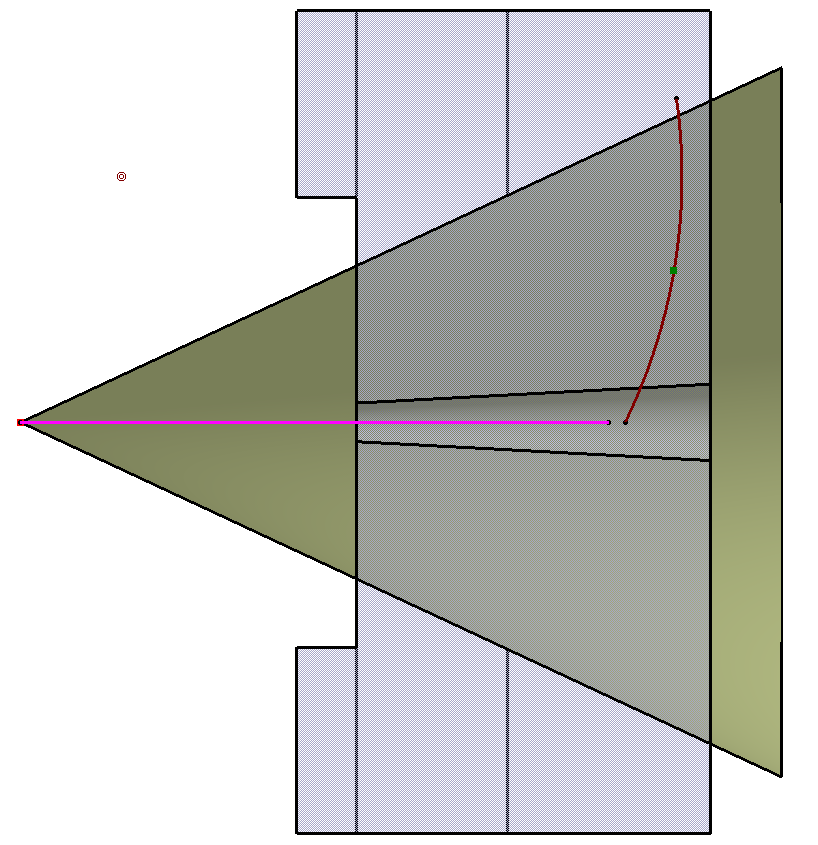
\includegraphics[width=0.7\textwidth]{pictures/RICH_construction.png}
%\caption{Схема детектора CBM RICH, сид сбоку. Жёлтый конус -- геометрический аксептанс.}
%\label{fig:RICHconstruction}
%\end{figure}

% ==============================================================================================
%  ____           _ _       _             
% |  _ \ __ _  __| (_) __ _| |_ ___  _ __ 
% | |_) / _` |/ _` | |/ _` | __/ _ \| '__|
% |  _ < (_| | (_| | | (_| | || (_) | |   
% |_| \_\__,_|\__,_|_|\__,_|\__\___/|_|   
%                                         
% ==============================================================================================

\subsubsection{Радиатор}\label{sec:CbmRichRadiator}

% 10 -> нескольких. Почему?! \todo

Разделение электронов и $\pi$-мезонов в диапазоне импульсов до нескольких~\GeVoverC{} требует низкого коэффициента преломления радиатора. Поэтому в CBM RICH планируется использование углекислого газа.
$CO_{2}$ имеет пороговый гамма-фактор $\gamma _{th} = 1 / \sqrt{1 - 1/n^{2}} = 31.6$, где $n = 1.0005$ --- коэффициент преломления для ближнего ультрафиолета при нормальных условиях. Максимальный черенковский угол составляет $\theta = arccos(1/n) = \SI{1.81}{\degree}$. Порог черенковского излучения для заряженных $\pi$-мезонов составляет $p = 4.41$~\GeVoverC{}, а для электронов и позитронов --- $p = 0.03$~\GeVoverC{}. При этом порог для каонов составляет $\approx 16$~\GeVoverC{}. Верхняя граница по импульсу составляет $\approx 10$~\GeVoverC{} и определяется тем, что кольца от электронов и $\pi$-мезонов должны быть дискриминированы по радиусу с эффективностью около 90\%.

Нижняя граница длин волн, пропускаемых $CO_{2}$, составляет 185~нм. Оценки показывают, что вклад сцинтилляции радиатора в общий счёт фотоэлектронов пренебрежимо мал.

% When designing a RICH detector ``one has to be extremely careful in matching the choice of (gas-)radiator with the sensitive wavelength range of the photon detection system'' [66]. In the case of the CBM-RICH, the low wavelength limit of the photomultiplier sensitivity (see section 3.4) coincides well with the absorption edge of $CO_{2}$ at $\approx 185$ nm (see section 6.2.1).

% Т.к. $CO_{2}$ не показывает высокого уровня сцинтилляции его часто добавляют в радиаторы, где другой газ является основным, в качестве гасящего газа. Ожидается около 5~фотонов/МэВ, в основном в синей области спектра. Энерговыделение в радиаторе порядка 1~\GeV{} ожидается при центральном $Au+Au$ столкновении, где рождается $\approx 1000$ минимально ионизирующих частиц, приводящих к $\approx 5000$ сцинтилляционных фотонов, летящих изотропно вдоль трека частицы. Если консервативно предположить, что 20\% фотонов достигает плоскости фотодетекторов и 25\% из них регистрируется, то в результате данного эффекта регистрируется дополнительно около $250$ фотонов, распределённых равномерно. При общем числе каналов порядка 55~000, указанный шум от сцинтилляции добавляет до 0.45\% ??? по всем каналам. Данный показатель находится в допустимом пределе и CBM RICH не теряет в эффективности.

% Due to the fact that $CO_{2}$ does not exhibit a high level of scintillation, it is often added to other radiator gases as quenching gas. Approximately 5 photons/MeV, mostly in the blue wavelength range, are expected [69]. An energy deposit in the radiator of $\approx 1$ GeV{} is expected for a central Au+Au collision with $\approx 1000$ minimum ionizing particles [6] leading to 5000 scintillation photons emitted isotropically along the particle tracks. This leads to $\approx 250$ measured additional photons distributed homogeneously over the photon detector plane when conservatively assuming that 20\% of the photons reach the photon camera with 25\% of them being detected. Given the total of 55 000 channels, noise from scintillation will add up to 0.45\% of all channels. This is well within the noise level that the CBM-RICH detector can tolerate without performance loss [6].

% ==============================================================================================
%   ____                             _                 
%  / ___| __ _ ___     ___ _   _ ___| |_ ___ _ __ ___  
% | |  _ / _` / __|   / __| | | / __| __/ _ \ '_ ` _ \ 
% | |_| | (_| \__ \   \__ \ |_| \__ \ ||  __/ | | | | |
%  \____|\__,_|___/   |___/\__, |___/\__\___|_| |_| |_|
%                          |___/                       
% ==============================================================================================

\subsubsection{Газовая система}\label{sec:CbmRichGasSystem}

% http://hepd.pnpi.spb.ru/hepd/articles/6.pdf
% Я так понял, система для прототипа сопадает с системой для всего детектора.

Закрытая газовая система сконструирована на основе опыта экспериментов STAR и PHENIX. Система автоматического регулирования поддерживает $CO_{2}$ при избыточном давлении 2~мбар. В контуре принудительной рециркуляции до 30\% газа ответвляется в систему очистки на основе активной меди и осушки для избавления от кислорода и влаги. Система мониторинга следит за попаданием параметров газовой системы в установленные пределы и запускает необходимые процедуры коррекции в случае выхода за эти пределы.

% ==============================================================================================
%  __  __ _                         
% |  \/  (_)_ __ _ __ ___  _ __ ___ 
% | |\/| | | '__| '__/ _ \| '__/ __|
% | |  | | | |  | | | (_) | |  \__ \
% |_|  |_|_|_|  |_|  \___/|_|  |___/
%                                   
% ==============================================================================================

\subsubsection{Система фокусировки}\label{sec:CbmRichMirrors}

Фокусировка черенковского света на фоточувствительные камеры достигается однократным отражением черенковских фотонов от двух сегментированных сферических зеркал радиусом 3~метра, расположенных на расстоянии 3500~мм от точки взаимодействия.
% Рассматривался также вариант с двойным отражением, при этом вторая группа зеркал была плоская.
Центры сферических поверхностей и сами зеркала расположены симметрично относительно горизонтальной плоскости, проходящей через ось пучка.
Зеркала полностью покрывают аксептанс детектора. Площадь каждого зеркала составляет приблизительно 7.5~м$^2$.
%Форма зеркал выбрана так, чтобы покрывать аксептанс без выполнения поворотов.
%При этом
Линия, соединяющая центр поверхности зеркал и центр сферы, наклонена вокруг оси~X приблизительно на \SI{10}{\degree} в направлении от пучка,
что позволяет разместить фоточувствительные камеры не только за пределами аксептанса, но и вывести их в зону слабого магнитного поля.
% На раннем этапе проектирования CBM RICH исходя из доступного пространства в общей экспериментальной установке было рассчитано, что фокусирующая система CBM RICH должна выполнять одно отражение с помощью двух сферических зеркал радиусом 3~метра, расположенных на расстоянии 3500~мм от точки взаимодействия.
Оптимизация формы зеркал подробно рассмотрена в главе~3. % \todo

% \todo на досуге подыскать ссылки
Для того чтобы выполнить требование к точности, зеркало такого размера технологически возможно изготовить только из сегментов. Прототипы сегментов тестировались на однородность и отражательную способность. Были выбраны зеркала, произведённые фирмой \mbox{JLO-Olomouc}, Чехия. Зеркала будут выполнены из SIMAX-стекла толщиной 6~мм и покрыты слоем $Al+MgF_{2}$ с внутренней стороны. Алюминий с покрытием хорошо отражает фотоны от видимого света до дальнего УФ. Слой $MgF_{2}$ используется как защитный слой с целью предотвращения появления пленки оксида алюминия, который поглощает ультрафиолет. Характерный размер сегмента --- 40--50~см. Каждое зеркало будет разделено на 40~сегментов, расположенных в четырёх горизонтальных рядах.

% Original English text
% The mirror tiles are made of a 6~mm thick SIMAX glass substrate front-coated with $Al+MgF_{2}$. Aluminium provides a good reflectivity in both the visible and the UV wavelength region down to below 200~nm. The $MgF_{2}$ layer is used as protective layer in order to prevent the formation of UV absorbing aluminium oxide. Mirror tiles from JLO Olomuc were successfully tested in a prototype (see section 5.1), characterised in terms of homogeneity [70] and reflectivity [71], and chosen to be used for the CBM-RICH detector.

% Далее рассматривается только одно, верхнее зеркало. Всё описание распространяется и на симметричное нижнее зеркало.

% Вообще есть целое направление, в котором люди занимаются тем, что оценивают и обычно стараются минимизировать material budget.


% \todo Не, ну вот это я бы оставил!
% Основная задача зеркал --- отвести черенковские фотоны в область, где они могут быть зарегистрированы фоточувствительной камерой, которую невозможно расположить напрямую на пути этих фотонов, т.е. в геометрической аксептансе. Это сделает работу последующих детекторов невозможным из-за вторичных частиц.
% Для того, чтобы фокусировать фотоны на камеру, расположенную за пределами аксептанса, необходимо, чтобы центр сферической поверхности располагался над осью пучка, а сами зеркала полностью покрывали акспетанс. Есть как минимум два варианта геометрии зеркал. В первом зеркало выполняется симметричным относительно горизонтальной плоскости и поворачивается вокруг оси X. При этом возникает зазор между двумя зеркалами, расширяющийся к краям (см. \figref{fig:MCgeoMirrorsEvolution}), но все зеркала составляются из сегментов двух типов. Более оптимальный способ --- выбрать правильную долю сферы так, чтобы зеркала стыковались без зазора. При этом зеркало получается несимметричным, а следовательно необходимо 4 типа сегментов.


%Для того, чтобы верхнее и нижнее зеркала стыковались без зазора необходимо 4~типа сегментов. Сегменты зеркала будут иметь размер около 40см$\times$40см.
% (точное значение указать невозможно, это ж не прямоугольник)

% Данный вопрос также затрагивается в \ref{sec:secMirrorsEvolution}
Ссылка на \figref{fig:MCgeoMirrorsEvolution} и секцию~\ref{sec:secMirrorsEvolution}.
% Вот в CBM будет правый вариант. \todo

% Полагая, что $\pi$-мезоны и электроны могут быть разделены с эффективностью до 90\% \todo при максимальном черенковском угле $\theta = arccos(1/n)$, 

% The separation of electrons and pions at momenta below 10~\GeVoverC{} requires a low refractive index of the radiator and therefore determines the radiator to be a gas. A $CO_{2}$ radiator is foreseen which has a threshold Lorentz factor of $\gamma _{th} = 1 / \sqrt{1 - 1/n^{2}} = 33.3$, given a refractive index of $n = 1.00045$ at a temperature of \SI{0}{\degreeCelsius}, a pressure of 1000~mbar, and a wavelength of 600~nm. The Cherenkov threshold is $p = 4.65$~\GeVoverC{} for charged pions and $p = 0.03$~\GeVoverC{} for electrons and positrons. The threshold for kaons is $\approx 16$~\GeVoverC{}. The saturated Cherenkov angle for ultrarelativistic particles is $\SI{1.72}{\degree}$. Assuming that pions can be separated from electrons up to 90\% of the maximum Cherenkov opening angle $\theta = arccos(1/n)$, electrons and pions can be separated up to $\approx$ 10~\GeVoverC{} with $CO_{2}$ as radiator gas.

% Явление chromatic absorption в $CO_{2}$ становится заметным только в области длин волн менее 200~нм и, следовательно, не ухудшает разрешения черенковского кольца.

% For $CO_{2}$, chromatic absorption becomes sizeable only in the region below 200 nm (see section 6.2.1) and does not deteriorate the Cherenkov ring resolution significantly as shown below.

% The mirror of the CBM-RICH detector is split into two parts above and below the beam pipe. Each mirror half is oriented towards a photon detection plane and part of a sphere with R = 3.00 m. The total area of the two mirror halves is $12.96 m^2$ . The mirror halves consist of 36 mirror tiles each arranged in four rows of nine tiles. The tiles themselves have a slightly trapezoidal shape in order to minimise gaps in between to 3~mm to~4 mm. Two different tile sizes are foreseen, 430/425.6 mm $\times$ 425~mm for the inner two rows and 425.5/412.5~mm $\times$ 425~mm for the outer rows.

% A tripod concept is foreseen for mounting the mirror tiles on an aluminum frame. Each mirror tile is glued to three actuators allowing for the precise alignment of the tiles in a sphere.

% Запятая? "При этом,"
% А это вообще так возможно? В полном детекторе сначала собрать с актуаторами, а затем заменить их на винты? И с чего это Вы взяли, что так будет?

Каждый сегмент зеркал будет крепиться на раме с помощью трёх винтов. При этом, в прототипе и при калибровочных запусках полномасштабного детектора могут использоваться моторизированные актуаторы, необходимые для оптимизации положения сегментов по ходу сеанса. Далее рассматривается возможность замены, с помощью специально разработанной процедуры, механизированных актуаторов на легкие опорные винты, что позволит сохранить оптимальную юстировку и снизить количество вещества в аксептансе.
% актуаторов без удалённого управления.
% Это позволяет корректировать положение отдельных сегментов между запусками пучка. \todo переформулировать
% Ожидается, что нет причин чтобы наклон долей зеркал поплыл после начальной юстировки

% В связи с такими-то причинами
% , корректируя отклонения от правильного положения, связанные с перемещениями точек механической опоры, находящейся в напряжённо-деформированном состоянии под собственным весом и весом зеркал. Также возможны перемещения в связи с термическим расширением рамы при изменении параметров окружающей среды в экспериментальном зале.

Метод CLAM~(\cite{CLAM}) позволяет оценивать неравномерность отклонений отдельных сегментов зеркал по результатам анализа фотографий отражённых прямых линий. Планируется применение данного метода для калибровки CBM RICH.

% Коллаборациями LHCb и COMPASS разработаны методы \todo, позволяющие выполнять...
% Для анализа в моделировании необходимо обеспечить возможность поворота отдельных сегментов зеркал вокруг заданных осей. В связи с этим была построена версия MC-модели, отличающаяся структурой объёмов и обеспечивающая возможность поворота отдельных сегментов зеркал вокруг заданных осей. Эта модель обсуждается в \ref{sec:secRICHgeoMirrorMis}.

% Для того чтобы минимизировать рождение вторичных частиц в материале опорных конструкций особое внимание отводится минимизации материала в аксептансе. Исходя из этого опоры зеркал проектируются так чтобы они имели минимальный вес при достаточной жёсткости.
% In order to reduce the production of secondary particles, the material budget of the RICH detector has to be kept low. The mirror support structure is therefore designed as a compromise between stability and light weight.

% ==============================================================================================
%   ____                               
%  / ___|__ _ _ __ ___   ___ _ __ __ _ 
% | |   / _` | '_ ` _ \ / _ \ '__/ _` |
% | |__| (_| | | | | | |  __/ | | (_| |
%  \____\__,_|_| |_| |_|\___|_|  \__,_|
%                                      
% ==============================================================================================

\subsubsection{Фотодетекторы}\label{sec:CbmRichCamera}

Фоточувствительная камера разрабатывается для регистрации одиночных фотонов с высокой эффективностью. Для успешной реконструкции событий необходима точная регистрация координат и времени прилёта каждого фотона.
% Task of the CBM-RICH photon camera is the detection of Cherenkov photons produced by charged particles in the gas radiator and reflected by the focusing mirror. The camera is developed for the detection of single photons with high efficiency. A precise measurement of position and time of arrival of each photon is required as input for the ring reconstruction algorithm discussed in section 2.5.3.
% Фоточувствительная камера CBM RICH состоит из двух половин, имеющих
Используется две камеры цилиндрической формы, расположенные над и под пучком в фокальной плоскости сферических зеркал. Черенковский свет, отражённый от верхнего зеркала, регистрируется верхней камерой. Соответственно, свет, отражённый от нижнего зеркала, регистрируется нижней камерой.
% The photon camera of the CBM-RICH detector consists of two parts, one above and one below the beam pipe in the focal plane of the spherical mirrors. The two photon detector planes are located in front of the CBM dipole magnet shielded by the magnet yokes. The Cherenkov rings from the upper mirror half will be projected onto the upper photon detector, rings from the lower mirror half onto the lower photon detector. Each of the two photon detector planes is divided into two parts in order to optimise the angle towards the mirror. Thus, the camera consists of four separated areas, so-called camera modules. Each module covers an area of 0.6~m $\times$ 1.0~m (height $\times$ width). The total active camera area is $2.4 m^{2}$.

В качестве фоточувствительных элементов будут применяться многоанодные фотоэлектронные умножители Hamamatsu H12700, см. секцию~\ref{sec:secMapmt}. Использование данной модели МА~ФЭУ не требует дополнительных фокусирующих элементов.
% The CBM-RICH design foresees the usage of commercially available multianode photomultiplier tubes (MAPMTs) as photon sensors. The use of Micro Channel Plate (MCP) sensors is considered as alternative [6]. Due to the good geometrical coverage of these sensor types, no focusing elements like lenses or Winston cones are envisaged.
% -------------------------------------------------------------------------------------------------------------------------------
% \todo
% Переработать, частичное дублирование того, что написано в секции про реализацию МАФЭУ в Билдере.
Один такой МА~ФЭУ имеет габариты 52$\times$52~мм$^2$. Для защиты камеры от магнитного поля будут использоваться экраны из магнитно-мягкого железа.
Планируется, что фоточувствительная камера будет составлена из (примерно сколько \todo) модулей, содержащих 2$\times$3 МА~ФЭУ. С учётом зазора в 1~мм между МА~ФЭУ для запаса по точности, размер модуля составляет 158мм$\times$105мм.

%\begin{figure}[H]
%\centering
%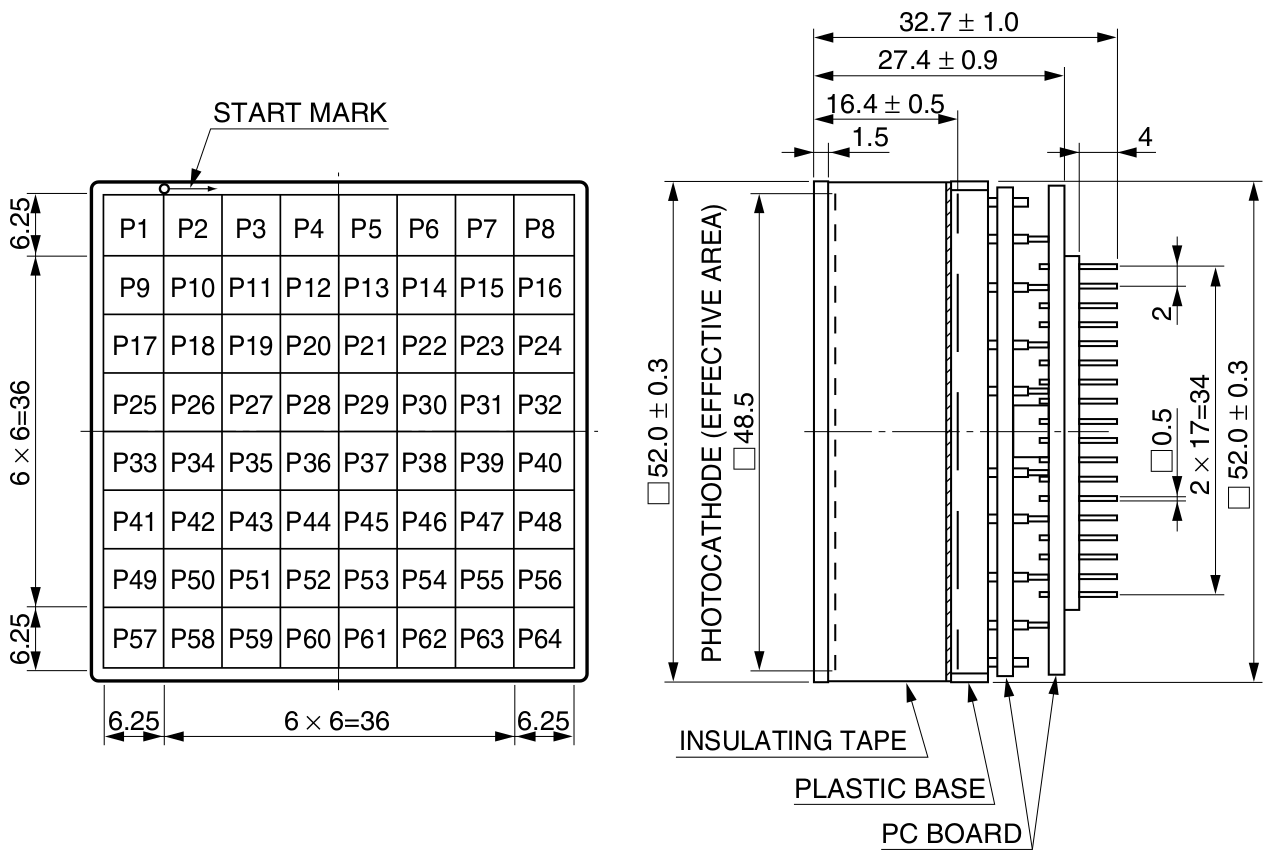
\includegraphics[width=0.7\textwidth]{pictures/H12700_drawing.png}
%\caption{Чертёж МА~ФЭУ H12700 из документации.}
%\label{fig:H12700drawing}
%\end{figure}
% -------------------------------------------------------------------------------------------------------------------------------

% В момент написания данной работы тестируется прототип модуля. \todo перетащить в 3-4-5 главу?
% разработке программ для FPGA, но имеются изготовленный прототип.
Помимо МА~ФЭУ в модуль входят 12~плат передней электроники DIRICH, одна плата, обеспечивающая питание, и одна плата концентрации данных. Механической основой модуля служит плата-адаптер, к которой с одной стороны подсоединяются МА~ФЭУ, а с другой --- все платы, см. также~\ref{sec:secRICHgeoCamera}. 

% CAD-модель и MC-модель модуля показаны на~\figref{fig:geoMCmodule}. \todo утащить

%\todo \textbf{Сообразить, где писать про систему считывания и сбора данных, что будет мотивировкой к главам 4 и 5. Здесь или в отдельной секции?}

Система считывания и сбора данных CBM~RICH подчиняется концепции, описанной в \todo. Исследованию прототипа этой системы посвящены главы~4~и~5.

% ==============================================================================================
%  ____       _            _                      _                     __   _                _ __  
% |  _ \  ___| |_ ___  ___| |_ ___  _ __      ___| |__   __ _ _ __     / /__| |__   ___  _ __| |\ \ 
% | | | |/ _ \ __/ _ \/ __| __/ _ \| '__|    / __| '_ \ / _` | '__|   | / __| '_ \ / _ \| '__| __| |
% | |_| |  __/ ||  __/ (__| || (_) | |      | (__| | | | (_| | |_     | \__ \ | | | (_) | |  | |_| |
% |____/ \___|\__\___|\___|\__\___/|_|       \___|_| |_|\__,_|_(_)    | |___/_| |_|\___/|_|   \__| |
%                                                                      \_\                      /_/ 
% ==============================================================================================

% \todo цифры из 1.3.1 надо давать после описания конструкции, а не до.

% Я погорячился насчет характеристик. без обсуждения вариантов и оптимизаций какие-то слова и картинки об эффективностях регистрации, средних парамаетрах колец и зависимости эффективности ID от импульса надо здесь дать.
% \todo что?!

\subsubsection{Характеристики CBM RICH}\label{sec:CbmRichChar}

%Вводное предложение о том, что рич восстанавливает кольца по хитам.

\textbf{Какая часть секции \ref{sec:secCbmRichOptimiz} идёт сюда?}

Восстановление колец в RICH выполняется по хитам, спроецированным на плоскость реконструкции.\\
В среднем 28~хитов на кольцо. \\
% откуда взялось это число? Сколько в прототипе? По моим результатам. (см. слайды с онлайн рич-митинга)
% см. прогресс репорт 2013, стр. 52
Средний радиус кольца составляет~4.5~см. \\
Средняя эллиптичность кольца равна~0.937. \\

% \todo Причесать.
% Уменьшение детектора
Стремление к уменьшению общей стоимости детектора привело к уменьшению его размеров. Количество зарегистрированных фотонов пропорционально длине радиатора вдоль пучка, а значит уменьшение детектора приводит к понижению его эффективности.
Так, например, HERA-b RICH (см. секцию~\ref{sec:HerabRich}) регистрирует 33~фотона на кольцо, в то время как в соответствии с моделированием в CBM будет регистрироваться 28~фотонов на кольцо.

То, насколько хорошо хиты выстраиваются на кольце зависит от углового разрешения детектора для черенковских фотонов. В работе~\cite{TDR_RICH, KOPFERDISS} подробно рассмотрены факторы влияющие на это разрешение. Показано, что основные вклады вносят: гранулярность камеры, неидеальности зеркала, многократное рассеяние излучающей частицы и хроматическая дисперсия черенковского света в радиаторе, отклонение траектории частицы от прямолинейной в паразитном магнитном поле.
Вклады многократного рассеяния и паразитного магнитного поля возрастают при уменьшении импульса. В качестве характерной величины приведём $\sigma = 0.38$~мрад для электронов с импульсом $p=8$~\GeVoverC{}.

%For 20 detected photons per Cherenkov ring and neglecting errors from the mirror quality, the overall error is calculated according to equation (2.11) to be σ = 0.38 mrad for p = 8 GeV/c corresponding to 1.3\% of the saturated Cherenkov opening angle for ultrarelativistic particles of 1.72° = 30.02 mrad.

\bigskip

Процедура восстановления события в CBM RICH детекторе схематично показана на~\figref{fig:StsRichReco}, подробнее см.~\cite{}.

% Дублирует кусок в секции sec:secReconstruction.
Реконструкция в CBM~RICH означает поиск колец по хитам в плоскости реконструкции. В контексте реконструкции можно рассматривать хит как загоревшийся пиксель МА~ФЭУ. Конус черенковских фотонов, после фокусировки зеркалами, пересекает поверхность фоточувствительной камеры, которая в общем случае может состоять из нескольких плоскостей. Первый этап реконструкции --- перевод хитов из плоскостей камеры в плоскость реконструкции. Затем выполняется поиск колец по хитам. В CbmRoot есть реализации нескольких алгоритмов поиска колец. Наибольший практический интерес представляет алгоритм распознавания колец черенковского излучения, основанный на проеобразовании Хафа и описанный в работах~\cite{RECOPEPAN, RECO2}. Реализация данного алгоритма была специально адаптирована для данных пучковых тестов, в которых ожидается одно кольцо на событие. Данный алгоритм реализован в классе \classname{CbmRichProtRingFinderHoughImpl}, унаследованном от \classname{CbmRichProtRingFinderHough} и далее от \classname{CbmRichRingFinder}. После этого определяются параметры кольца и далее осуществляется реконструкция треков частиц с применением информации с других детекторов.

\begin{minipage}[t]{0.495\textwidth}
\begin{figure}[H]
\centering
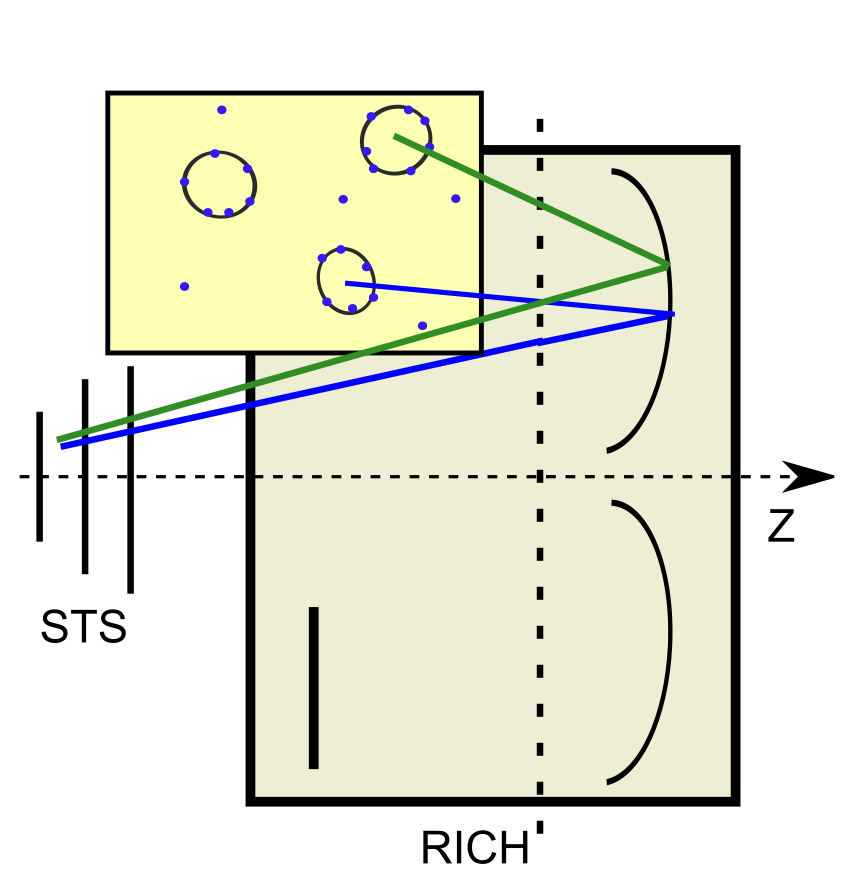
\includegraphics[width=0.95\textwidth]{pictures/STS_RICH_reco.png}
\caption{Сначала независимо выполняется реконструкция треков в STS и восстановление колец в RICH. Затем трек STS пропагируется до зеркала и рассчитывается пересечение отражённого продолжения с плоскостью реконструкции RICH. Последний этап --- сопоставление продолженных треков с центрами колец.}
\label{fig:StsRichReco}
\end{figure}
\end{minipage}
\begin{minipage}[t]{0.495\textwidth}
Вследствие большой множественности в центральных столкновениях в одном событий в RICH регистрируется 65~колец.
% В эксперименте CBM из точки взаимодействия $Au+Au$ при 25~\GeVperNucl{} в аксептанс RICH попадает около 1000 заряженных частиц. При этом частота первичных взаимодействий достигает 10~МГц. Эти условия диктуют следующие требования. Реконструкция колец в CBM RICH должна выполняться в среде высокой плотности частиц, многие из которых являются заряженными $\pi$-мезонами с высоким импульсом. В дополнение к этому, фотоны, рождённые в точке взаимодействия конвертируются в материале детектора в пары $e^{+} e^{-}$. В результате одном событии в RICH регистрируется около 65 колец.
На \figref{fig:CbmRichOneEvent} приведено изображение на одной плоскости реконструкции от одного смоделированного события $Au+Au$ 25~\GeVperNucl{}. Плотность хитов в одиночном событии достигает значения 0.5 хитов/см$^{2}$. Алгоритмы реконструкции должны быть достаточно быстрыми, рассчитанными на достаточно широкий диапазон количества хитов на кольцо (от~5 до~40) и способными работать с эллиптической формой колец.
% The main challenge for the ring reconstruction is the high hit multiplicity in heavy ion collisions.
% For central Au+Au collisions at 25 AGeV, around 1000 charged particles are produced in the RICH acceptance, many of them being charged pions with high momenta. In addition, photon generated in the interaction are converted to e± pairs by conversion processes in the detector material or even in the target. This results in ≈ 65 rings per event on the RICH camera. Figure 2.9 shows the response of the upper two camera modules to Au+Au collisions at 8 AGeV and 25 AGeV. The maximum hit density is ≈ 0.5 hits/cm2/event.
% Other challenges are the high interaction rate of up to 10 MHz requiring fast reconstruction algorithms, the varying number of hits per ring from 5 to 40, and the elliptic shape of the rings in the outer regions of the camera (see below).
\end{minipage}

\begin{figure}[H]
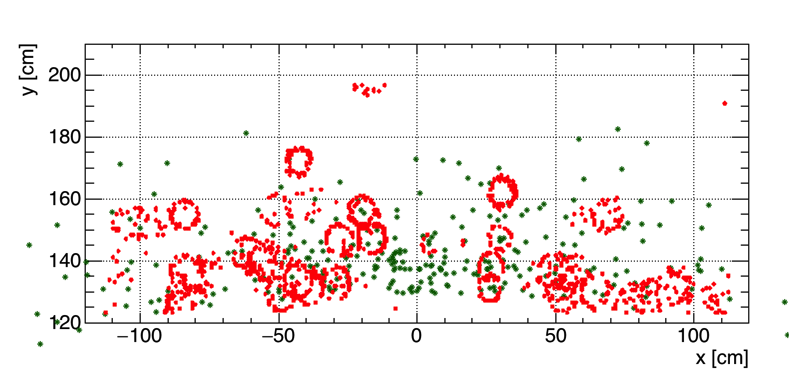
\includegraphics[width=0.9\textwidth]{pictures/CbmRichOneEvent.png}
\caption{Типовое событие (UrQMD, 25~\GeVperNucl{}) в одной фотодетектирующей плоскости RICH. Красные точки --- хиты RICH, зелёные --- продолжения треков STS.}
\label{fig:CbmRichOneEvent}
\end{figure}

В результате обильных симуляций получены характеристики, показанные на~\figref{fig:RICHeff}, \ref{fig:InvMassSpectra} и табл.~\ref{tabl:RICHchar}.
% \todo развернуть

\begin{figure}[H]
\begin{minipage}[t]{0.495\textwidth}
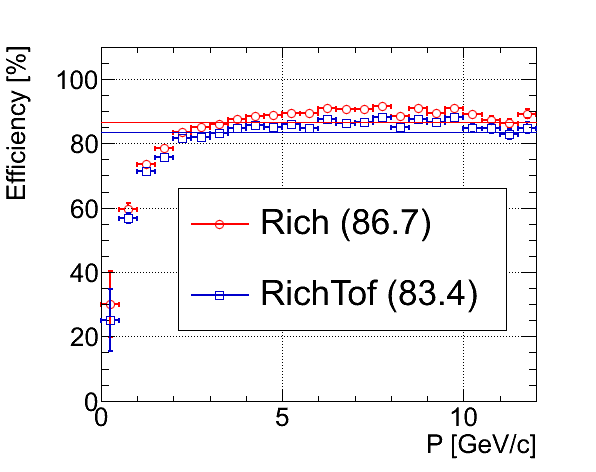
\includegraphics[width=0.95\textwidth]{pictures/RICHeff1.png}
\end{minipage}
\begin{minipage}[t]{0.495\textwidth}
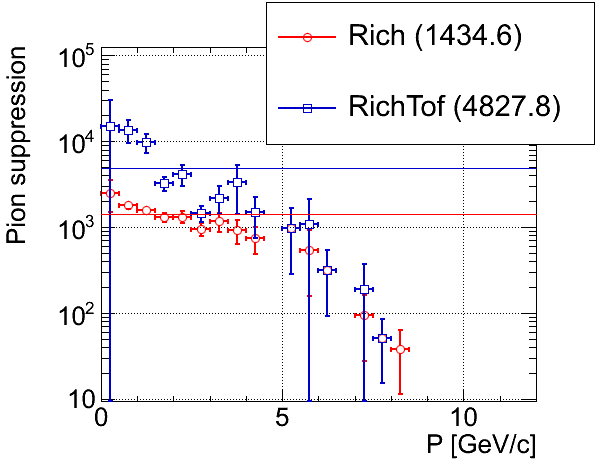
\includegraphics[width=0.95\textwidth]{pictures/RICHeff2.png}
\end{minipage}
\begin{minipage}[t]{0.495\textwidth}
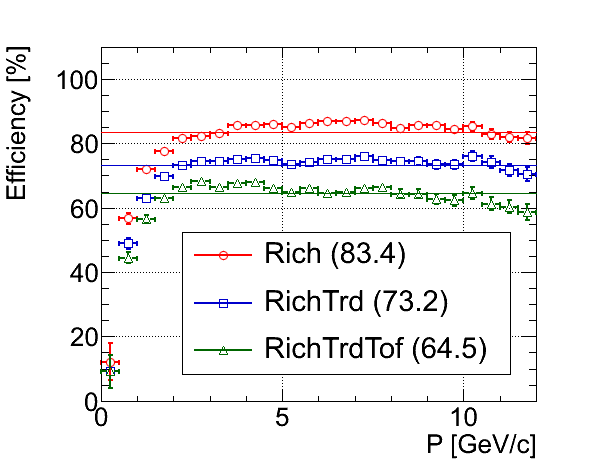
\includegraphics[width=0.95\textwidth]{pictures/RICHeff3.png}
\end{minipage}
\begin{minipage}[t]{0.495\textwidth}
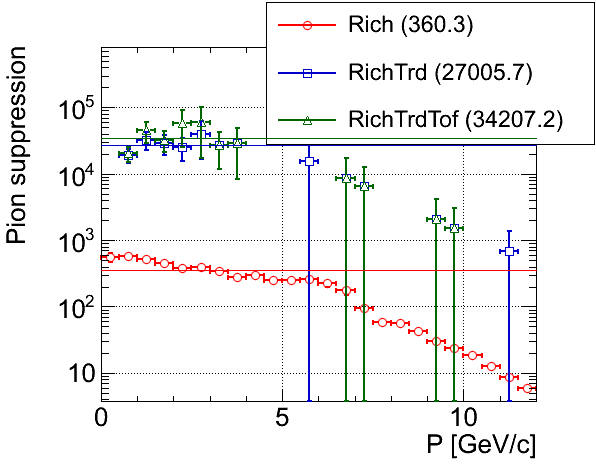
\includegraphics[width=0.95\textwidth]{pictures/RICHeff4.png}
\end{minipage}
\caption{Сверху --- 8~\GeVperNucl{}, снизу --- 25~\GeVperNucl{}.}
\label{fig:RICHeff}
\end{figure}

\begin{table}[H]
\caption{Отношение сигнал-шум (S/B), вклад $e^{+}e^{-}$-пар из распада Далица и конверсии гамма-квантов в полный комбинаторный фон в процентах и вклад ложно идентифицированных $\pi^{\pm}$ в процентах от полного числа электронов после применения всех критериев отбора. Для достижения чувствительности к лёгким векторным мезонам необходимо чтобы физические источники сигнала доминировали над фоном, что требует фактор подавления $\pi$-мезонов более 5000. Таблица взята из~\cite{TDR_RICH}.}
\label{tabl:RICHchar}


% Signal-to-background ratios, the contribution of physical background in percent to the total number of pairs in combinatorial background
% and the contribution of misidentified $\pi^{\pm}$ in percent to the electron sample after applying all cuts.

% \todo проверить перевод
% S/B, contribution of physical background in percent of the total number of pairs in the background and the contribution of misidentified $\pi^{\pm}$ in percent of the electron sample after application of all background rejection cuts.
% A pion suppression of $>5000$ is needed to have the background dominated by physical sources and to reasonably access low mass vector mesons.

\begin{tabular}{ | p{0.28\linewidth} p{0.07\linewidth} p{0.07\linewidth} p{0.07\linewidth} p{0.07\linewidth} p{0.07\linewidth} p{0.07\linewidth} p{0.1\linewidth} | }

\hline
Фактор подавления $\pi$ & 100 & 500 & 1000 & 2500 & 5000 & 10000 & идеальн. \\
\hline
\hline

& & & 8~\GeVperNucl{} & & & & \\
\hline
$\omega$: $S/B$ & 0.012 & 0.14 & 0.27 & 0.47 & 0.67 & 0.83 & 0.89 \\
\hline
$\phi$: $S/B$ & 0.001 & 0.015 & 0.03 & 0.05 & 0.07 & 0.12 & 0.14 \\
\hline
Физич. фон, \% & 1.8 & 18.4 & 34.7 & 55.6 & 69.8 & 79.5 & 86.9 \\
\hline
Ложн. идентиф. $\pi^{\pm}$, \% & 83.5 & 53.4 & 36.4 & 19.3 & 10.6 & 5.7 & 0.0 \\
\hline
\hline

& & & 25~\GeVperNucl{} & & & & \\
\hline
$\omega$: $S/B$ & 0.005 & 0.05 & 0.10 & 0.19 & 0.24 & 0.26 & 0.30 \\
\hline
$\phi$: $S/B$ & 0.002 & 0.02 & 0.04 & 0.07 & 0.10 & 0.12 & 0.14 \\
\hline
Физич. фон, \% & 1.8 & 18.7 & 35.9 & 57.1 & 69.1 & 76.9 & 86.0 \\
\hline
Ложн. идентиф. $\pi^{\pm}$, \% & 83.9 & 52.7 & 36.0 & 18.5 & 10.4 & 5.2 & 0.0 \\
\hline

\end{tabular}

\end{table}

% Чё-то написать

\begin{figure}[H]
\begin{minipage}[t]{0.495\textwidth}
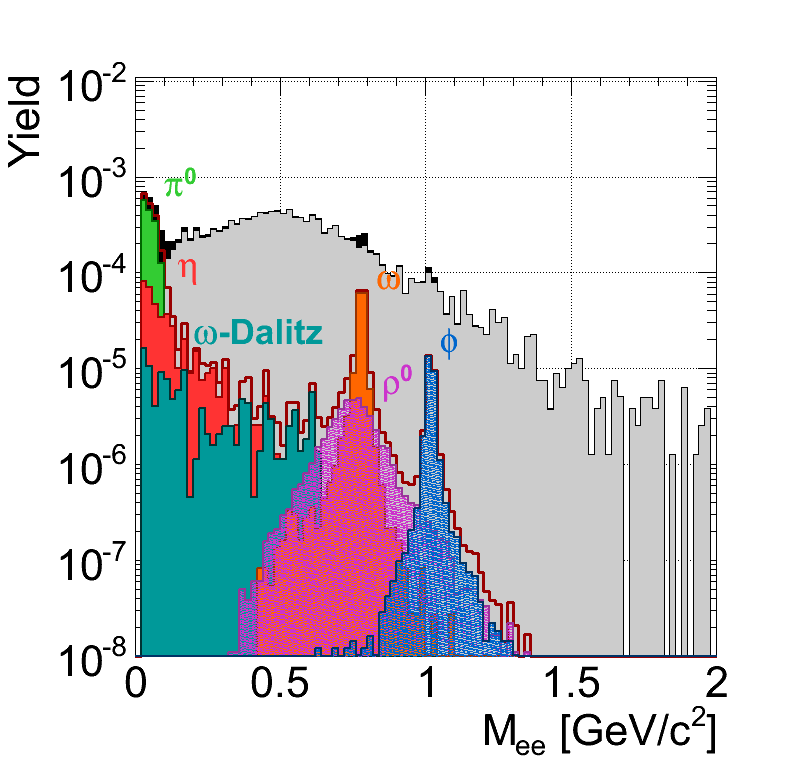
\includegraphics[width=0.95\textwidth]{pictures/InvMassSpectr1.png}
\end{minipage}
\begin{minipage}[t]{0.495\textwidth}
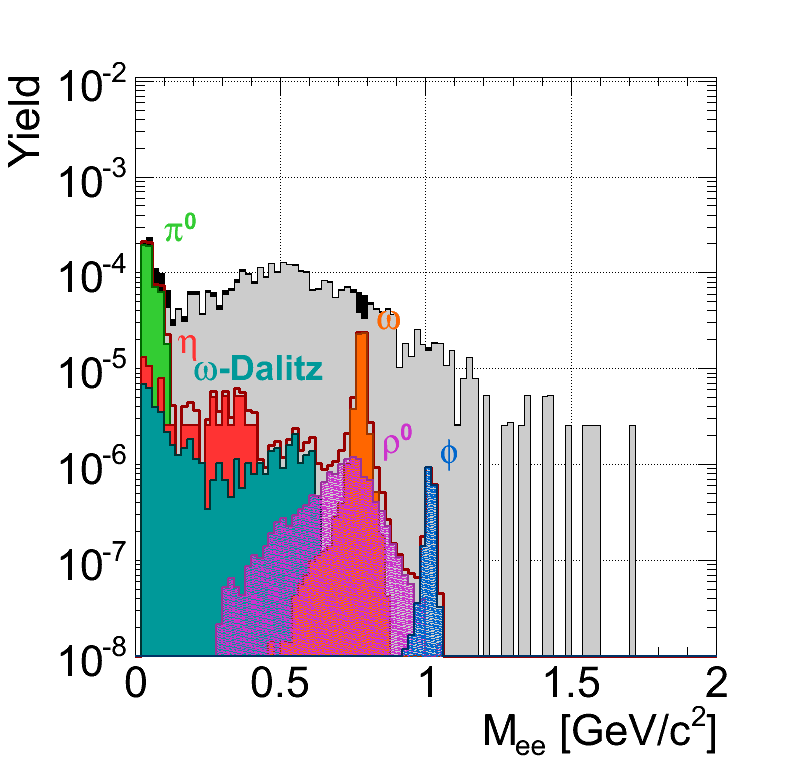
\includegraphics[width=0.95\textwidth]{pictures/InvMassSpectr2.png}
\end{minipage}
\caption{Смоделированные спектры инвариантных масс диэлектронов после применения всех критериев отбора для энергии 8~\GeVperNucl{} (SIS100, 100000 событий, слева) и 25~\GeVperNucl{} (SIS300, 200000 событий, справа). Серым цветом показан фон. Рисунок взят из~\cite{TDR_RICH}.}
\label{fig:InvMassSpectra}
\end{figure}

% Invariant mass spectra of simulated di-electrons after application of all background rejection cuts. Central Au+Au collisions were simulated at 8 AGeV (left) and 25 AGeV beam energy (right) corresponding to SIS100 and SIS300 scenarios, respectively. Colored histograms represent the hadronic cocktail, the grey histogram the background. The left plot is based on 100 000 events, the right plot based on 200 000 events. Figures taken from CBM RICH TDR.
